\documentclass[tikz]{standalone}
\usepackage{tikz}
\usepackage{pgfplots} % loads tikz which loads pgf
\pgfplotsset{compat=1.18}
\usetikzlibrary{arrows, arrows.meta, calc, shapes, positioning, patterns, 
decorations.pathreplacing, decorations.pathmorphing, shapes.geometric, shapes.symbols, shapes.arrows, 
datavisualization, datavisualization.formats.functions, automata, fit, angles, quotes, decorations.markings, 3d, backgrounds}
\tikzset{>=latex} % for LaTeX arrow head
\colorlet{myred}{red!85!black}
\colorlet{myblue}{blue!80!black}
\colorlet{mycyan}{cyan!80!black}
\colorlet{mygreen}{green!70!black}
\colorlet{myorange}{orange!90!black!80}
\colorlet{mypurple}{red!50!blue!90!black!80}
\colorlet{mydarkred}{myred!80!black}
\colorlet{mydarkblue}{myblue!80!black}
\tikzstyle{xline}=[myblue,thick]
\def\tick#1#2{\draw[thick] (#1) ++ (#2:0.1) --++ (#2-180:0.2)}
\tikzstyle{myarr}=[myblue!50,-{Latex[length=3,width=2]}]
\usepackage[american,siunitx]{circuitikz}

\begin{document}
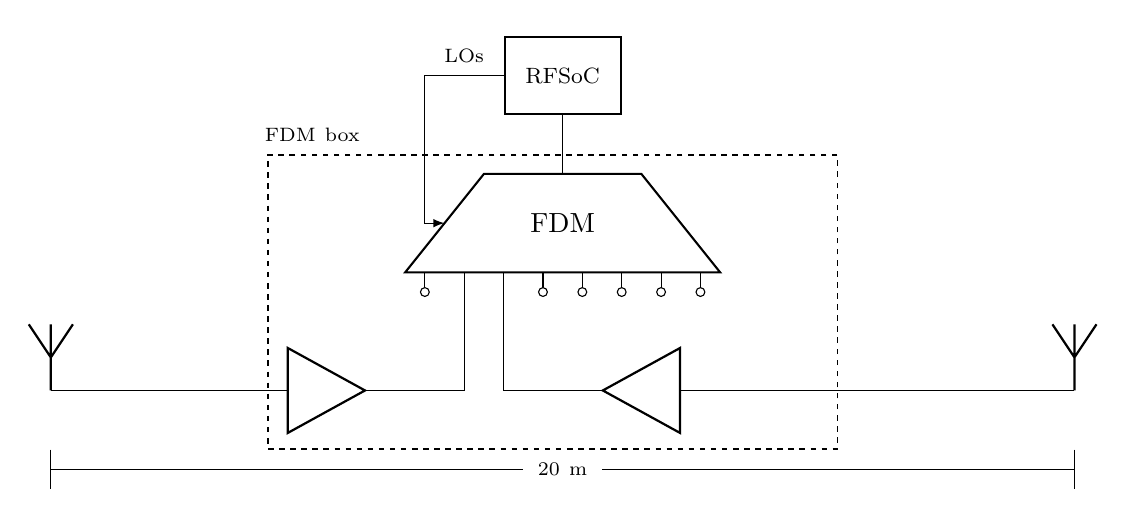
\begin{tikzpicture}
	% Paths, nodes and wires:
	\node[shape=rectangle, draw, line width=0.75pt, minimum width=1.474cm, minimum height=0.974cm] at (17.5, 7){} node[anchor=center, align=center, text width=1.094cm, inner sep=5.75pt] at (17.5, 7){\footnotesize RFSoC};
	\draw[line width=0.75pt] (15.5, 4.5) -- (19.5, 4.5) -- (18.5, 5.75) -- (16.5, 5.75) -- cycle node[anchor=center] at (17.5, 5.125){$\text{FDM}$};
	\draw (15.75, 4.25) -- (15.75, 4.5);
	\draw (16.25, 4.25) -- (16.25, 4.5);
	\draw (17.5, 5.75) -- (17.5, 6.5);
	\draw (15.75, 5.25) |- (16.75, 7);
	\draw[latex-] (16, 5.125) -| (15.75, 5.25);
	\node[shape=rectangle, minimum width=2.465cm, minimum height=0.715cm] at (16.25, 7.25){} node[anchor=center, align=center, text width=2.077cm, inner sep=6pt] at (16.25, 7.25){\scriptsize LOs};
	\draw (16.75, 4.25) -- (16.75, 4.5);
	\draw (17.25, 4.25) -- (17.25, 4.5);
	\draw (17.75, 4.25) -- (17.75, 4.5);
	\draw (18.25, 4.25) -- (18.25, 4.5);
	\draw (18.75, 4.25) -- (18.75, 4.5);
	\draw (19.25, 4.25) -- (19.25, 4.5);
	\node[ocirc, rotate=90] at (19.25, 4.25){};
	\node[ocirc, rotate=90] at (18.75, 4.25){};
	\node[ocirc, rotate=90] at (18.25, 4.25){};
	\node[ocirc, rotate=90] at (17.75, 4.25){};
	\node[ocirc, rotate=90] at (17.25, 4.25){};
	\node[ocirc, rotate=90] at (15.75, 4.25){};
	\node[dinantenna] at (24, 3){};
	\node[dinantenna] at (11, 3){};
	\draw (15, 3) -- (16.25, 3) -| (16.25, 4.25);
	\draw (16.75, 4.25) -| (16.75, 3) -- (18, 3);
	\draw (19, 3) to[amp, mirror] (18, 3);
	\draw (14, 3) to[amp] (15, 3);
	\draw (11, 3) -- (14, 3);
	\draw (19, 3) -- (24, 3);
	\draw (11, 2) -- (17, 2);
	\draw (18, 2) -- (24, 2);
	\draw (24, 2.25) -| (24, 1.75);
	\draw (11, 2.25) -| (11, 1.75);
	\node[shape=rectangle, minimum width=2.465cm, minimum height=0.715cm] at (17.5, 2){} node[anchor=center, align=center, text width=2.077cm, inner sep=6pt] at (17.5, 2){\scriptsize 20 m};
	\node[shape=rectangle, draw, line width=0.5pt, dash pattern={on 2pt off 2pt}, minimum width=7.232cm, minimum height=3.732cm] at (17.375, 4.125){};
	\node[shape=rectangle, minimum width=2.465cm, minimum height=0.715cm] at (14.75, 6.25){} node[anchor=west, align=left, text width=2.077cm, inner sep=6pt] at (13.5, 6.25){\scriptsize FDM box};
\end{tikzpicture}
\end{document}